The \gls{id}~\cite{ATLASPaper} is designed to provide good track reconstruction,
precise momentum resolution and both primary and secondary vertex measurements
(see Section~\ref{sec:primary-vertex}) above a nominal $\pt$ threshold of
0.5~GeV and within the pseudorapidity $|\eta| < 2.5$. The ID is 6.2~m long and
has a radius of about 1.1~m, it is surrounded by a solenoidal magnetic field of
2~T. Its layout is schematized in Figure~\ref{fig:id} and, as can be seen, it is
composed of three sub-detectors.

At the inner radius the \emph{pixel detector} measures charged particles with
silicon sensors with a minimum and maximum size of $50 \times 400$~$\mu$m$^2$
and $50 \times 600$~$\mu$m$^2$ respectively.

In the middle of the ID the \gls{sct} is designed to give eight precision
measurements per track which contribute to determine the primary and secondary
vertex position and momentum measurements. The silicon sensors are 80~$\mu$m
pitch micro strips.

The last layer of the ID is the \gls{trt}, it contributes to tracking and
identification of charged particles. It consists of drift (straw) tubes, 4~mm in
diameter with a 31~$\mu$m wire in the center of each straw, filled with a gas
mixture. These tubes substantially act like proportional counters where the tube
is the cathode and the wire is the anode and set to ground. When a charged
particle cross one tube, leaves a signal; the set of signals in the tubes,
reconstructs to a track which represents the path of the crossing object. The
space between the straw tubes is filled with material with a different
dielectric constant than the inside, this causes charged particles crossing the
boundaries to emit transition radiation thus leading to some straw to have a
much stronger signal. The transition radiation depends on the Lorentz $\gamma$
factor which in turn depends on the energy and the mass of the particles.
Lighter particles will have higher transition energy and stronger signal in the
straw tubes. This allows to distinguish between electrons (the lightest charged
particle) and single hadrons (pions), for instance, tracks with several strong
signal straw, can be identified as belonging to electrons.

An additional layer, the \gls{ibl}, was recently added in the region between the
beam pipe and the inner pixel layer (B-layer). It is designed to increase the
tracking robustness by replacing damaged parts of the pixel B-layer and
increasing the hit redundancy with higher luminosity. In addition, being closer
to the beam pipe it increases the impact parameter measurement
precision~\cite{IBL}.

\begin{figure}[!h]
  \centering
    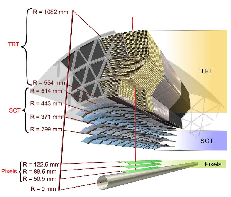
\includegraphics[width=.8\linewidth]{inner_detector}
    \caption{Schematic view of a charged track of 10~GeV $\pt$ that traverses
      the different ID sub-detectors. After traversing the beryllium pipe, the
      track passes through the three cylindrical silicon-pixel layers, the four
      layers of silicon-microstrip sensors (SCT) and the approximately 36 straws
      contained in the TRT within their support structure~\cite{ATLASPaper}.}
    \label{fig:id}
\end{figure}
%%% Local Variables:
%%% mode: latex
%%% TeX-master: "../search_for_DM_LED_with_ATLAS"
%%% End:
